\documentclass[crop, tikz]{standalone}
\usepackage{tikz}
\usetikzlibrary{arrows, shapes, decorations.pathmorphing, backgrounds, positioning}

\definecolor{mygreen}{rgb}{0,0.6,0}
\definecolor{mymauve}{rgb}{0.58,0,0.82}

\tikzset{
  snakearrow/.style={-stealth, mymauve, thick,
    decoration={snake, pre length=0.01mm, segment length=2mm, amplitude=0.3mm, post length=1.5mm}, decorate},
  zigzagarrow/.style={-stealth, mygreen, thick,
    decoration={zigzag, pre length=0.01mm, segment length=2mm, amplitude=0.3mm, post length=1.5mm}, decorate},
}

\begin{document}
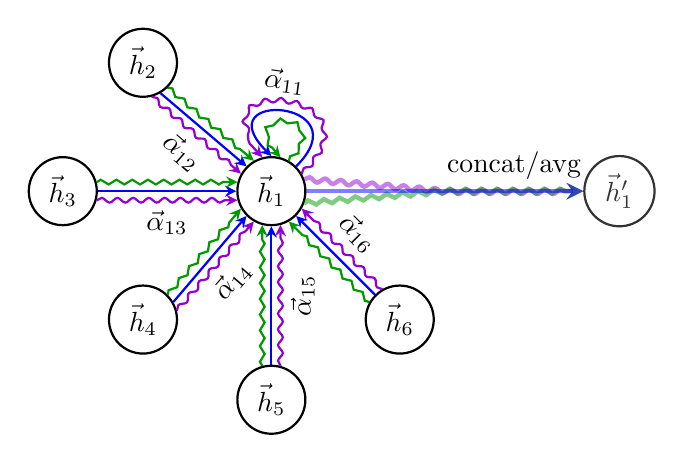
\begin{tikzpicture}
  \node[circle, draw, thick] (h1) {$\vec{h}_1$};
  \node[circle, draw, thick, above left=of h1] (h2) {$\vec{h}_2$};
  \node[circle, draw, thick, left=5em of h1] (h3) {$\vec{h}_3$};
  \node[circle, draw, thick, below left=of h1] (h4) {$\vec{h}_4$};
  \node[circle, draw, thick, below=5em of h1] (h5) {$\vec{h}_5$};
  \node[circle, draw, thick, below right=of h1] (h6) {$\vec{h}_6$};

  % per neighbor: snake/straight/zigzag arrows at fanned-out anchor angles
  \foreach \n/\sa/\sb/\sc/\ia/\ib/\ic/\idx/\side in {%
      2/285/300/315/150/135/120/12/below, 3/-15/0/15/195/180/165/13/below,
      4/15/30/45/240/225/210/14/below, 5/75/90/105/-75/-90/-105/15/below,
      6/120/135/150/-30/-45/-60/16/above} {
    \draw[snakearrow] (h\n.\sa) -- node[sloped, \side, black] {$\vec{\alpha}_{\idx}$} (h1.\ia);
    \draw[-stealth, blue, thick] (h\n.\sb) -- (h1.\ib);
    \draw[zigzagarrow] (h\n.\sc) -- (h1.\ic);
  }

  \draw[snakearrow] (h1.30) to[looseness=7] node[sloped, above, black] {$\vec{\alpha}_{11}$} (h1.105);
  \draw[-stealth, blue, thick] (h1.45) to[looseness=9] (h1.90);
  \draw[zigzagarrow] (h1.60) to[looseness=20] (h1.75);

  \node[circle, draw, thick, right=10em of h1, opacity=0.8] (hp) {$\vec{h}_1'$};
  \coordinate[right=5em of h1] (A);

  \draw[snakearrow, opacity=0.5, ultra thick] (h1.20) -- (A) -- (hp);
  \draw[zigzagarrow, opacity=0.5, ultra thick] (h1.-20) -- (A) -- (hp);
  \draw[-stealth, blue, opacity=0.5, ultra thick] (h1.0) -- (A) -- node[black, above, opacity=1.0] {concat/avg} (hp);
\end{tikzpicture}
\end{document}
